%!TEX root = ../../csuthesis_main.tex
\chapter{系统功能实现与实验验证}

\section{系统整体运行流程}

本系统依靠Carla仿真平台及其Python接口实施开发,重点围绕视觉目标检测,跟踪及行为意图识别展开融合工作,从而创建起一套具有即时性与可视化特征的自动驾驶感知子系统,此系统能够在Carla环境里达成目标感知,意图推断以及图形界面交互这样一种完整的循环过程,进而给后面的风险决策或者辅助控制供应先验方面的输入信息。

系统以 client\_bounding\_boxes.py 作为主控脚本,它的运作流程包含如下一些重要步骤:

仿真环境初始化: 程序先通过 carla.Client 和 Carla 仿真服务创建起联系,再把预先指定好的地图场景(诸如 Town10)给加载进来,接着生成代表我方车辆(egovehicle)以及周围环境中的交通流,设置好摄像头之类的传感器之后开启同步模式。

实时图像获取与处理: 车辆前置RGB摄像头持续采集画面帧图,系统凭借Carla原生的投影功能从场景当中获取每辆车的3D边界框,并把它投影到图像平面上,以此当作检测输入。

目标选择与跟踪处理: 系统通过图像中心最近原则选定一个主目标当作跟踪对象,再用DeepSORT算法实施跨帧关联,守住稳定的目标ID。
行为意图识别: 依靠跟踪到的信息,再加上目标速度,运动方向以及中心点位移的改变情况,用物理建模的办法来做行为趋向判断,给出“靠近”“远离”“危险靠近”之类的表述。

可视化与数据记录: 系统把全部边界框,目标编号以及意图分析文字及时画到主界面上,用户可以用键盘来操控车辆行驶,而且系统每隔一定帧数就会把图像和标注信息自动存成数据集,以供后面训练和评价时使用。

图像渲染环节利用Pygame完成,该部分把图像帧,边界框,速度信息,追踪ID以及意图结果等相关元素加以整合,然后一并绘制到显示窗口上,从而生成出清晰易懂的运行界面,为了给后续的模型训练及效果回溯给予支撑,系统内部设置有自动保存图像帧和标注信息的功能,它会按照规定的间隔将图像以及包含边界框和速度信息的JSON格式文件存入本地数据集文件夹之中。而且,系统还加入了针对各个模块执行时间的统计功能,每当一帧处理结束之后就会输出各个阶段所花费的时间,当系统运行过一定数量的帧数之后,就会把所有时间段的详细信息整理成一张CSV表格并保存下来,方便使用者展开性能方面的分析与改良工作。

通过以上流程的达成,本系统既在仿真环境下做到了从感知到认识直至警报的全过程闭合,又有着较好的可视化表现能力和运行稳定程度,从而给后面章节里的功能演示以及性能评价形成牢靠根基。

\section{界面展示}

系统基于 pygame 实现实时渲染窗口,在 Windows 系统上运行稳定,图像帧率维持在约 8~10 FPS。在主界面中,用户可清晰看到如下信息:

\textbf{•前视图图像帧:}显示本车前方道路环境、其他车辆等元素;

\textbf{•目标边界框:}每个检测到的车辆被标注为 3D 投影框;

\textbf{•跟踪目标编号:}被追踪目标在框上方显示 Tracked ID;

\textbf{•意图分析结果:}在跟踪目标框的上方显示当前系统判断的意图(如“危险靠近”、“目标远离中”等);

\textbf{•速度信息显示:}在边界框上标记目标当前速度(单位:m/s);

\textbf{•系统状态输出:}在终端控制台实时输出当前帧耗时、目标状态等信息,辅助调试与评估。

用户能够用键盘来操控本车的行为(比如油门,刹车,转向等),以此考察系统处于各种驾驶状态时的感知鲁棒性,要想验证本系统在Carla仿真平台上的运行情况,本节通过一组功能界面截图表现系统的重要功能模块以及动态交互过程,在系统运行期间,各个模块相互协作去执行车辆环境感知,目标筛选,轨迹追踪和行为意图判断,从而创建起稳定的视觉处理及风险提示体系。

\begin{figure}[H]
    \centering
    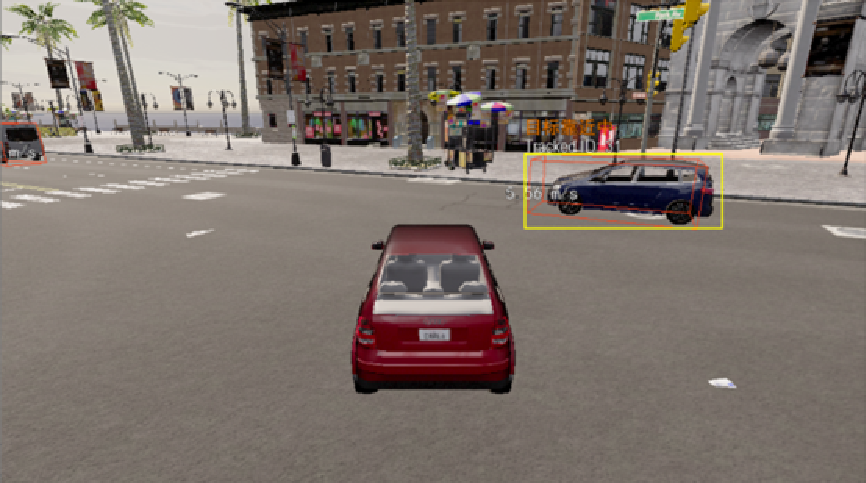
\includegraphics[width=0.8\textwidth]{images/图13 意图识别演示图(目标靠近).pdf}  % 引用转换后的 PDF 文件
    \caption{意图识别演示图(目标靠近)}
    \label{fig:example_image}  % 可用于引用此图片
\end{figure}

\begin{figure}[H]
    \centering
    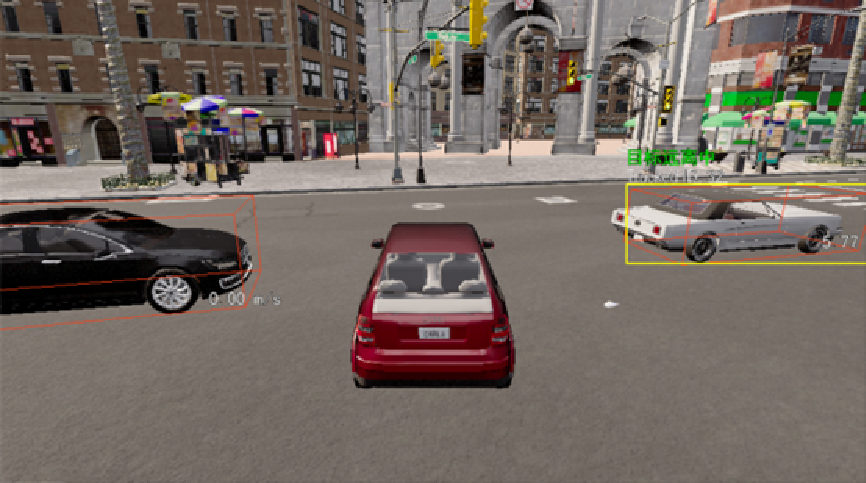
\includegraphics[width=0.8\textwidth]{images/图14 意图识别演示图(目标远离).pdf}  % 引用转换后的 PDF 文件
    \caption{意图识别演示图(目标远离)}
    \label{fig:example_image}  % 可用于引用此图片
\end{figure}

\begin{figure}[H]
    \centering
    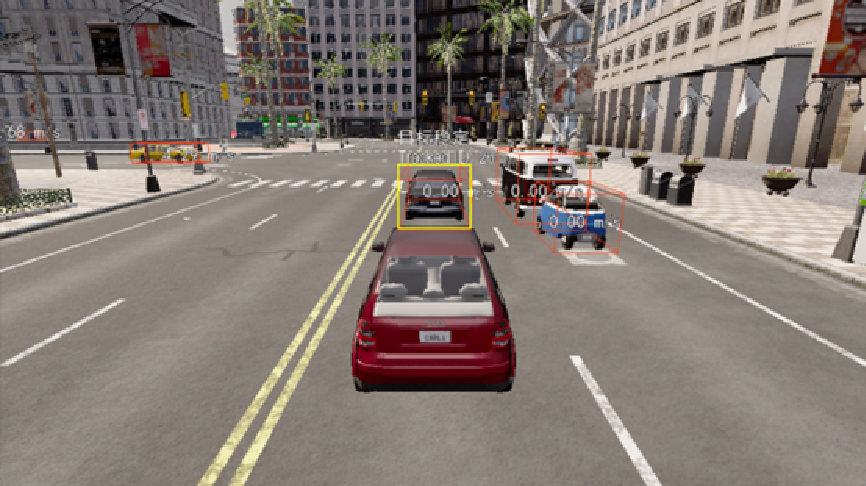
\includegraphics[width=0.8\textwidth]{images/图15 意图识别演示图(目标稳定).pdf}  % 引用转换后的 PDF 文件
    \caption{意图识别演示图(目标稳定)}
    \label{fig:example_image}  % 可用于引用此图片
\end{figure}

\section{用户交互与运行控制}

本系统设计时,充分考量到用户的交互体验及控制便利性,通过键盘操作结合即时图像反馈塑造起相对完备的人机交互机制,此系统主要依靠Pygame库来达成交互接口,从而让用户得以在仿真运行期间随时操控车辆运动,变更观察视角并查看感知成果。

车辆控制上,用户凭借键盘按键就能达成油门,制动,转向以及手刹这些基本驾驶行为,按一下W键就可以让车向前行驶,而S键则负责倒车,A/D键分别用来向左转和向右转,Space键被设定为手刹功能,ESC键能随时停止仿真运行,这样做是为了保证系统在用户结束的时候可以平稳地释放资源,关掉所有的传感器和窗口,系统会在每一次的循环里去读入键盘输入,并把它转化成Carla的控制指令,以此来做到对车辆持续不断的控制。

在感知交互上,用户通过主界面可直接看到每帧图像里感知与识别的成果,系统会自动画出车辆边界框,而且在被跟踪目标的框体上面显现其ID号以及行为意图判断结果,所有信息都是即时刷新的,这有益于用户知晓系统当下的感知状况和意图识别判断,当发生高风险情形(诸如危险靠近)的时候,系统就用红色高亮文字作出警告,以此来提升用户的关注度,进而达成辅助驾驶提醒的目的。

而且,系统具备自动数据采集与保存功能,可以随时把图像帧和标注信息记录到后台,不用人为参与,这个机制有益于之后的离线模型训练和性能考量,加强了系统的拓展性和工程应用价值,用户可以通过设置参数来指定数据采集的频次和储存形式,从而符合各种实验的需求。

本系统在用户交互设计上做到简洁明晰且操作灵活,再加上Carla仿真平台稳固的底层支撑,就形成起一个具有真实驾驶控制体验以及智能感知反馈能力的测试平台,可以有效地支撑相关算法的开发验证工作。


\begin{figure}[H]
	\centering
	\makebox[\textwidth]{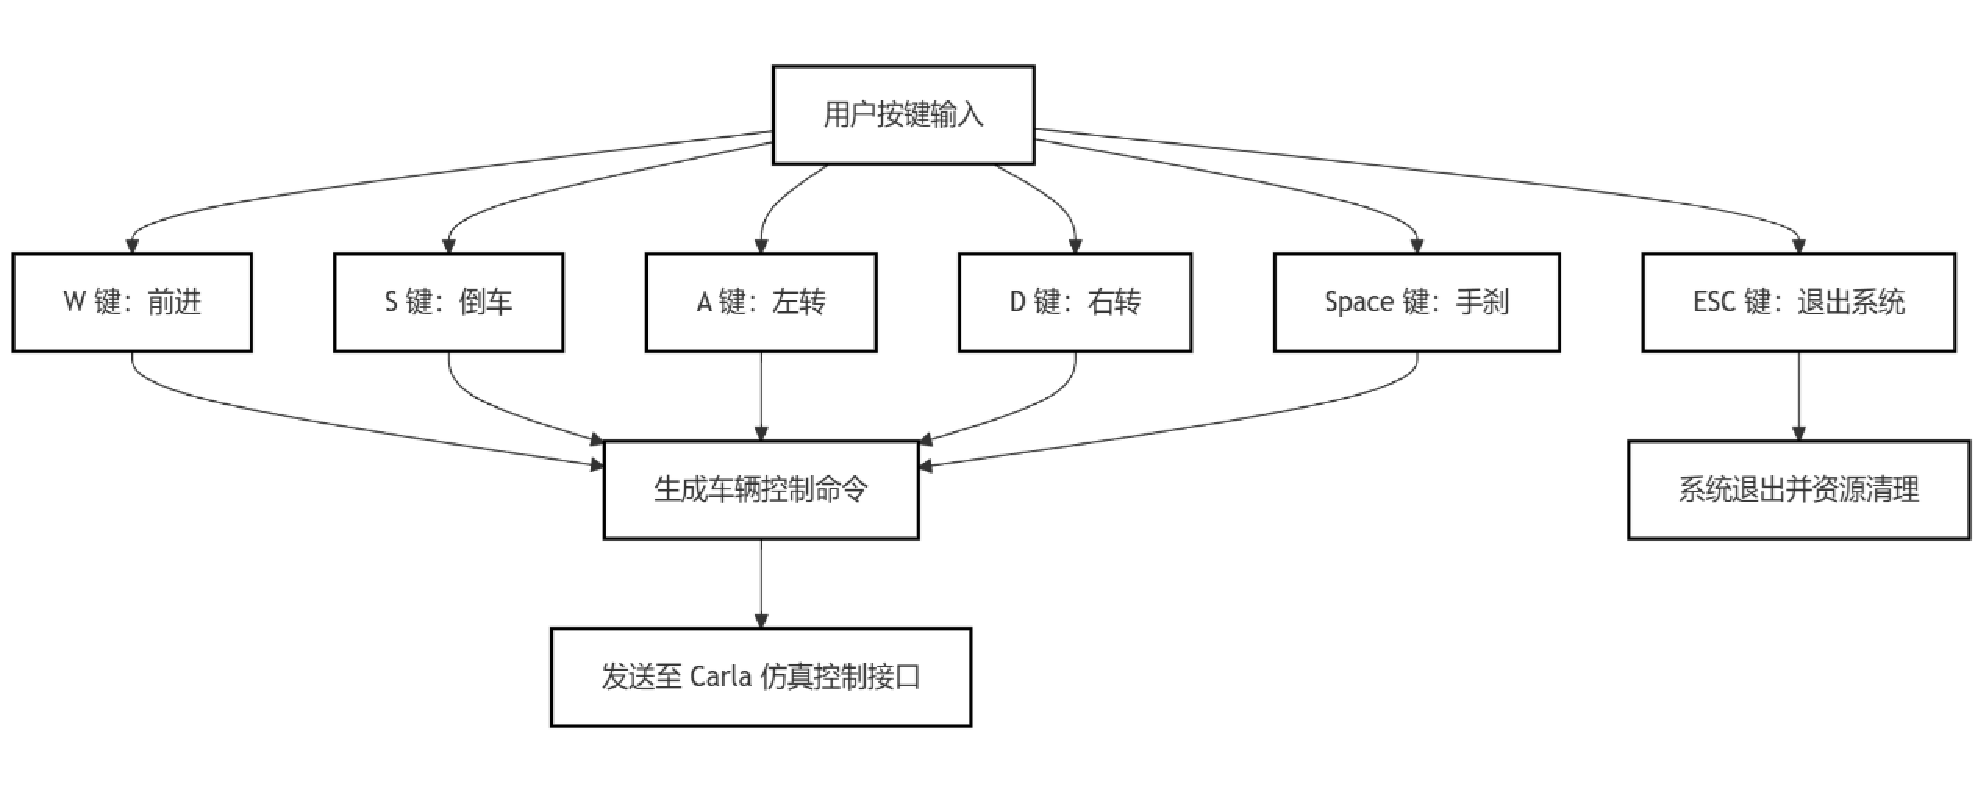
\includegraphics[width=1.2\textwidth]{图16 用户键盘控制映射关系示意图.pdf}}
	\caption{用户键盘控制映射关系示意图}
	\label{fig:example_image}
\end{figure}


\begin{tabular}{l l}
%  \verb|\songti| & {\songti 宋体} \\
%  \verb|\heiti| & {\heiti 黑体} \\
%   \verb|\kaiti| & {\kaiti 楷体}
\end{tabular}
